\documentclass[a4paper,11pt]{report}
\usepackage[T1]{fontenc}
\usepackage[utf8]{inputenc}
\usepackage{lmodern}
\usepackage[francais]{babel}
\usepackage{hyperref}
\usepackage{titlesec}
\usepackage{graphicx}
\usepackage{titling}

\titleformat{\chapter}{\normalfont\huge}{\thechapter.}{20pt}{\huge\it}
\setlength{\parindent}{4em}
\setlength{\parskip}{1em}

\title{\textbf{Compte rendu de projet} \\ Implémentation d’un algorithme de reconnaissance faciale en Python}
\author{THIEN NHAT Van et REVEST Florent\\\textit{2MICB 2015-2016}}

\pretitle{%
  \begin{center}
  \LARGE
  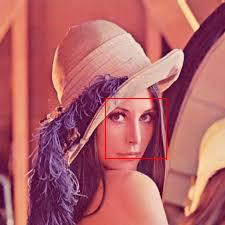
\includegraphics[width=6cm,height=6cm]{lenaDetected.jpg}\\[\bigskipamount]
}
\posttitle{\end{center}}

\begin{document}

\maketitle
\tableofcontents

\begin{abstract}
	Ce compte rendu présente l'expérience acquise dans le cadre de l'UF Projet de 2ème année Modélisation, Informatique, Communications de l'INSA Toulouse. Ce projet a consisté à comprendre et implémenter un algorithme de reconnaissance faciale efficace: la méthode Viola Jones. Nous décrirons ici les grandes lignes de son fonctionnement et de son implémentation. Le travail de programmation associé peut se trouver à l'adresse suivante :

\href{http://github.com/FlorentRevest/ViolaJones}{http://github.com/FlorentRevest/ViolaJones}.
\end{abstract}

\chapter{Introduction}
	Les machines programmables ont rapidement révolutionné la résolution de tâches simples et mécaniques, ou du moins mathématiquement formalisable. Pourtant on leur objecte souvent leur incapacité à résoudre des problèmes « humains », une catégorie de problèmes qui nous semble très simples et qui sont pourtant si complexes à formaliser en langage machine.

	L’un de ces problèmes est celui de la vision. Il semble évident pour un humain de reconnaître un objet ou une distance à l’aide du signal reçu par son nerf optique mais pourtant il serait bien incapable de l’expliquer. Dès lors, si la résolution est impossible à expliquer elle semble également impossible à formaliser.

	Les applications de la vision sont pourtant nombreuses : 
\begin{itemize}
\item En sécurité. E.g: avec la reconnaissance de piétons devant une voiture autonome
\item En médecine. E.g : pour reconnaître une tumeur dans une image.
\item En logistique. E.g : pour lire des adresses sur des enveloppes dans un centre de tri. (OCR)
\item En robotique. E.g : un robot/drone suivant un objet
\item etc...
\end{itemize}

	Dans les années 60, les chercheurs ont cherché à développer des méthodes rigides de description d’image, par exemple reconnaître un carré en décrivant un carré dans le code source. Ces méthodes se sont très vites montrées insuffisantes car pas assez adaptables à différents problèmes en situation réelles.

	Prenons l’exemple des problèmes de reconnaissance faciale. Essayer de décrire les caractéristiques d’un visage en terme d’yeux, de nez, de bouche et de cheveux dans une image qui est un tableau de pixels serait bien trop difficile. Depuis les années 70, toute sorte de méthodes statistiques ont été développées mais bien souvent leur temps de calcul était trop long pour faire de la reconnaissance « temps réel », par exemple sur un flux vidéo continu.

	En 2001, deux chercheurs des Mitsubishi Electric Research Labs à Cambridge, Paul Viola et Michael Jones ont publié un papier nommé « Rapid Object Detection using a Boosted Cascade of Simple Features » dans lequel ils définissent un algorithme de reconnaissance faciale maintenant connu sous le nom de « Méthode Viola Jones ».

	Très vite cette méthode s’est imposée dans de nombreuses applications industrielles en raison de sa simplicité et de sa rapidité. Par exemple la bibliothèque OpenCV (Open Computer Vision) d’Intel offre une implémentation open-source en C++ de la méthode Viola Jones qui a depuis été utilisée par de très nombreux projets.

	Le but de notre projet a été de comprendre cette méthode en détail et de fournir une implémentation open-source simple et didactique en Python pour documenter le sujet. Nous reviendrons sur ces deux axes dans les parties \textbf{La méthode Viola Jones} \textit{(théorique)} et \textbf{Notre implémentation} \textit{(pratique)} ensuite nous évoquerons l’organisation du développement dans le binome dans la partie \textbf{Organisation du travail}.

\chapter{La méthode Viola Jones}
	La reconnaissance faciale de Viola Jones se découpe en deux parties : une période d’apprentissage et une période de classification. Souvent ces deux parties sont découplées car l’apprentissage est long mais n’a besoin d’être exécute qu’une seule fois. La classification exploite les données de l’apprentissage pour rapidement détecter un visage dans une image inconnue.


\section{L’apprentissage}


	L’algorithme d’apprentissage est dit \textit{supervisé} car il exploite une large base de donnée d’exemples déjà \textit{labellisés}, par exemple quelques milliers d’images contenant un visage et quelques milliers d’images ne contenant pas de visages. De nombreuses bases de données de visages normalisés existent déjà pour faciliter le travail des chercheurs en reconnaissance faciale.

	La méthode Viola Jones exploite l’algorithme d’\textit{AdaBoosting} (pour Adaptive Boosting) pour \textit{s’entraîner} à découvrir des caractéristiques spéciales des visages. Le Boosting est une famille d’algorithme d’apprentissage machine entraînant un large ensemble de \textit{classifieurs faibles} pour construire un \textit{classifieur fort}.

	Le classifieur fort détermine à une large échelle si une matrice de pixels appartient à la classe « visage » ou à la classe « non visage » mais sa décision est faite à partir de la somme de très nombreux classifieurs faibles dont chacun a une décision pratiquement aléatoire (statistiquement les succès des classifieurs faibles sont à peine plus haut qu’un demi, c’est à dire que ceux du hasard).

	Les statistiques ainsi extraites permettent d’implémenter le programme classifieur.


\section{Le classifieur}


	La seconde étape de la méthode consiste à exploiter les structures de données fournies par l’AdaBoosting pour détecter un visage. Nous allons ici fournir une explication détaillée de chaque étape en allant du plus large au plus détaillé. Nous utiliserons les termes technique anglais originaux pour faciliter la compréhension du code.
	Une interprétation plus visuelle de ces informations peut être regardée en parallèle de la lecture à l’adresse: \href{https://vimeo.com/12774628}{https://vimeo.com/12774628}


\paragraph{Window:}
	Le classifieur ne connaît pas à l’avance la position et la taille du (ou des) visage(s) présent(s) dans l’image. Pour cette raison il va s’exécuter à toute les positions et tailles raisonnablement possibles dans l’image à tester. On définit ainsi une « \textit{window} » comme étant une fenêtre de test ayant une position et une taille et dans laquelle tous les calculs décrits ci dessous seront réalisés. L’apprentissage fournit des données pour une fenêtre de taille définie (20x20 dans notre implémentation),  il faudra donc normaliser les calculs pour cette taille.


\paragraph{Cascade:}
	Dans la visualisation vidéo fournit plus tôt, la fenêtre est visualisable par le carré rouge qui balaye la fenêtre. On remarque qu’il s’attarde plus ou moins sur certaines zones de l’images, ceci est dû à l’exécution de la \textit{cascade} qui peut être plus ou moins longue. Une cascade est une série de \textit{stages} testés les uns à la suite des autres. La window contient un visage si et seulement si tous les stages sont validés. Pour cette raison on arrête le calcul de la cascade de stage dès qu’un stage est négatif. Les zones ne contenant clairement pas de visage sont rapidement « court-circuité » dès les premiers stages. La cascade utilisée dans notre implémentation est faite de 20 stages.


\paragraph{Stage:}
	Un stage est une étape de calcul pouvant être valide ou pas. La validité du stage est déterminée par la comparaison d’une somme des évaluations des \textit{trees} sous-jacents avec un seuil, le \textit{stage threshold}. Si l’évaluation a un résultat supérieur au threshold alors le stage est valide. 


\paragraph{Tree:}
	Chaque stage contient un ensemble d’arbres binaires dont les nœuds sont des \textit{classifieurs faibles} et dont les feuilles ont une valeur. Un \textit{tree} est exploré en évaluant chaque classifieur des nœud depuis la racine. Le classifieur décide de l’exploration gauche ou droite de l’arbre binaire et donc de la valeur finale de l’arbre lorsqu’on arrive à une feuille.


\paragraph{Classifieur de feature:}
	Le classifieur évalue une \textit{Haar Feature} et la compare à un seuil, le \textit{node threshold}. Si l’évaluation de la feature est inférieure au seuil alors on explore l’arbre à gauche, sinon à droite.


\paragraph{Haar feature:}
	Finalement, les haar features constituent la plus petite composante de calcul de notre classifieur. C’est aussi, sans doute, la partie la plus intéressante de la méthode. Vous pouvez voir ci dessous une représentation de deux features se prêtant bien à l’interprétation visuelle. 

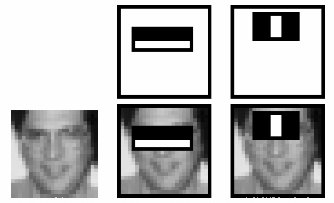
\includegraphics[width=300pt]{features.png}

	Une feature est un ensemble de rectangles définis dans le référentiel de la window de la cascade et ayant chacun un certain poids. Concrètement, il existe une infinité de features possibles, surtout avec des extensions comme celles de Lienhart qui rajoutent un « tilt » c’est à dire une rotation de la feature. Notre cascade n’en contient « que » quelques milliers et sans tilt. On évalue une feature en calculant la combinaison linéaire des poids de chaque rectangle avec la luminosité moyenne de l’image dans ce rectangle. Ce calcul donne une valeur qui sera ensuite exploitée par le classifieur. Dans l’illustration ci dessus on peut imaginer que la première feature correspond à la différence de luminosité entre l’ombre causée par les sourcil et les yeux. La feature de gauche pourrait correspondre à la luminosité du nez en comparaison aux zones extérieures des yeux mais toute les features ne s’interprètent pas aussi clairement.


\paragraph{Image intégrale:}
	Le calcul d’une luminosité moyenne dans un carré de taille n a une complexité évoluant en O($n^2$). Cela veut dire que le temps de calcul des features Haar et donc de la cascade peut rapidement devenir très long et donc difficilement s’adapter à du flux d’image vidéo. Une astuce de la méthode Viola Jones pour ramener ce calcul à une complexité constante O(1) est de définir une image intégrale comme étant une image dont chaque pixel contient la somme de tous les pixels à la gauche et au dessus de sa position. Ainsi, la somme des pixels dans un rectangle (x, y, width, height) peut s’obtenir avec la formule :  pix[x+width][y+height] +pix[x][y]-pix[x+width][y]-pix[x][y+height].

	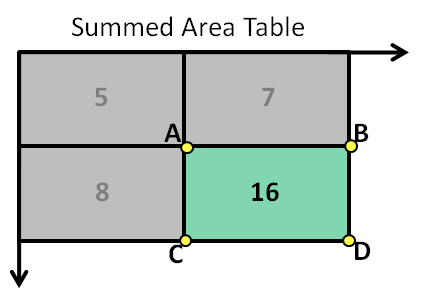
\includegraphics[width=300pt]{integral-image.png}

\par
	Il est vrai que le vocabulaire employé prend un certain temps à être adopté et l’imbrication de tous ces concepts est d'abord difficile à interpréter mais pour clarifier le processus nous pouvons résumer le classifieur comme étant un programme exploitant une succession d’étapes entraînées par l’apprentissage. Chaque étape contient un ensemble de \textit{caractéristiques} insignifiantes mais dont la somme donne une valeur qui définit la présence ou l’absence du visage.

\chapter{Notre implémentation}
	Une fois la méthode comprise il a fallu la réaliser. Pour la rapidité et la concision d’écriture nous avons choisi d’utiliser le langage Python. Le code de notre implémentation est disponible \href{https://github.com/FlorentRevest/ViolaJones}{ici}.

	Nous n’avons pas eu le temps d’explorer en détail la partie apprentissage de Viola Jones donc nous n’avons qu’un classifieur exploitant les données apprises par la bibliothèque OpenCV. La cascade d’OpenCV se trouve dans le fichier haarcascade\_frontalface\_alt2.xml au format xml. Il nous a donc fallu utiliser une bibliothèque de parsing de xml pour récupérer la structure dans un arbre. Cette partie est faite à l’aide du module lxml.

	L’ouverture facile d’images de tout formats a également été rendue possible à l’aide d’un module externe nommé PIL pour Python Imaging Library. On charge dans PIL l’argument de la commande puis on convertir l’image RGB en niveau de gris en associant au pixels verts un poids plus important pour émuler la vision humaine. La conversion de gris se fait selon la formule $G = (30*R+59*V+11*B)/100$ provenant également d'OpenCV.

	L’image intégrale est stockée à l’aide d’entiers de précision infinie, ce qui est facile à faire en Python. On y associe également une image intégrale au carré qui sert au calcul de la variance de l’image, utilisé pour un facteur de normalisation de la variance exploité par l’apprentissage d’OpenCV.

	Le classifieur est fait d’un ensemble de méthode d’évaluation des différentes étapes susmentionnées. Le découpage a été réalisé pour faciliter l’encapsulation et pour pouvoir facilement lire le code est l’explication théorique côte à côte.

	À la fin de l’exécution nous « simplifions » la liste de rectangles détectés pour supprimer d’éventuelles redondances de multiples détections imbriquées. Ensuite nous utilisons les méthodes de PIL pour dessiner les contours des visages détectés et les afficher à l’utilisateur.

\chapter{Organisation du travail}
	Nous sommes tous les deux habitués à travailler ensemble en programmation et avons donc une expérience du travail collaboratif qui nous a aidé à réaliser le projet sans grande difficulté. Cependant, pour faciliter le travail, nous avons cette fois ci prévu d’utiliser des outils de travail collaboratif comme Git pour garder un historique de révisions du code. 

	Pour travailler indépendamment, il nous a fallu découper le classifieur en un ensemble de petites fonctions indépendantes et facilement testables, par exemple le parsing du xml, le calcul de l’image intégral, la simplification des rectangles, l’affichage du résultat, les itérations sur la structure de donnée de la cascade et finalement le calcul des features Haar (qui a pris le plus de temps).

	La partie la plus difficile du projet a été de déboguer le calcul des features Haar, pour cela nous avons dû procéder incrémentalement et comparer les traces d’exécution de notre classifieur avec celui d’OpenCV. Compte tenu de l’imbrication de concepts et de la quantité de données produites il a été vraiment complexe de trouver la cause des problèmes que nous rencontrions.
	
\chapter{Conclusion}
		Ce projet a été une occasion fantastique d’approfondir nos connaissances informatique dans le domaine de l’apprentissage machine, de la vision par ordinateur et du traitement d’image. Nous avons pu prendre le temps de comprendre et documenter un algorithme de recherche omniprésent en industrie que beaucoup de personnes utilisent sans le comprendre via, notamment, OpenCV.

	Toutefois les choix didactiques que nous avons fait pour clarifier le code ont rendu l’execution plus lente que prévu. En effet, le classifieur d’OpenCV est capable de s’exécuter en moins d’un vingt-cinquième de seconde en utilisant par exemple du parallélisme pour le calcul de chaque feature ou du GPGPU avec Cuda. De plus l’implémentation compilée en C est sensiblement plus rapide que notre implémentation Python. Par conséquent, nous obtenons des temps de détection de 9 secondes sur une image de 512x512 pixels. Ce temps n’est pas acceptable pour du traitement temps réel mais ce sont des problèmes d’implémentation et non de la méthode.
\end{document}
